\documentclass{report}
\usepackage{graphicx} % Required for inserting images
\usepackage{geometry}
\geometry{a4paper,left=20mm,right=20mm,top=20mm,bottom=25mm}
\usepackage{imakeidx}
\usepackage{wrapfig}
\usepackage{subfigure}
\usepackage{hyperref}
\hypersetup{
    colorlinks=true,
    linkcolor=blue,
    filecolor=magenta,      
    urlcolor=blue,
    pdftitle={Overleaf Example},
    pdfpagemode=FullScreen,
    }

\makeindex

\title{\textbf{Heat and fluid flow in 3D Printers \\ Additive Manufacturing}}
\author{\Large{Nikshay Jain}\\MM21B044}
\date{April 2023}

\begin{document}

\maketitle
\tableofcontents

\chapter{Overview to 3D Printing}
\section{What is Additive Manufacturing/3D Printing?}
Additive manufacturing (3D Printing) is the process of formation of a three-dimensional object from a digital CAD model. It can be done in various processes in which material is joined, deposited, or solidified using computer controls, with the material being added together (such as plastics, liquids or powder grains being fused), typically layer by layer.

\section{Steps involved:}
\begin{enumerate}
    \item \textbf{Modelling:}
    
    It all starts from a 2D model in computer which are 3D printable, created with a computer-aided design (CAD) package or via a 3D scanner. CAD models can be saved in the 'stereolithography' file format (.stl).
    
    However, .stl is not used directly for additive manufacturing because it generates large file sizes of topology-optimized parts and lattice structures due to the large number of surfaces involved. A newer CAD file format, the Additive Manufacturing File format (AMF) is introduced to store information using curved triangulations.
    
    \item \textbf{Printing:}

    Most CAD applications produce errors to be repaired before printing in output files, like holes, noise shells, overhang issues, etc. It is then fed into a slicer converting model to thin layers and giving a G-code (numerical control programming language) file having instructions for the printer to interpret.
    \\The printer usually has a resolution describing layer thickness and X–Y resolution is given in dots per inch (dpi) or micrometre $(\mu)$. Typical layer thickness is around $100 \mu$ (250 DPI), although some machines can print layers as thin as $16 \mu$ (1,600 DPI).
    
    \item \textbf{Finishing:}
    
    The printer-produced resolution and surface finish are sufficient for some applications, however, post-processing and finishing methods allow for benefits such as greater dimensional accuracy, smoother surfaces, and other modifications such as colouration.
    \\Subtractive methods for surface finishing like sanding, and bead blasting, are generally employed. Annealing makes the internal bonds better due to recrystallisation thereby giving better strength, impact resistance and improved mechanical properties. But, due to the shrinkage of material in these processes, its not helpful when the dimensionality is important.
    
\end{enumerate}

The 3 steps above enumerate the manufacturing processes of a specimen superficially. Let's begin a detailed discussion on the manufacturing processes i.e. the printing for the product in the upcoming chapters.

\chapter{Fluid \& Heat flow in 3D Printers}

\section{Parts of 3D Printer to focus on:}
\begin{enumerate}
    \item Filament
    It is a coil of thermoplastic or a composite that comes in various diameters. The solid filament is fed through the printer and then into the extruders where it is melted and then extruded in liquid state which resolidifies after falling on the printing base.
    
    \item Extruder
    
    It is the component in 3D printers that holds the filament in place and controls the amount being fed into the hot end. They have stepper motors to control the movement of solid filament.

    \item Hot end

    It is the part where the filament is melted and sent to the nozzle.
    It comprises a feed tube (to guide the filament from the extruder to heat sink), a heatsink, thermal barrier tube with a heat break to melt the filament, and the nozzle to push it out to the printing base.

    \item Barrel
    It is the part of the extruder that contains the hot end and the nozzle. It is the component of the 3D printer that heats up and melts the plastic filament, allowing it to be extruded through the nozzle.

    \item Print head

    It is the part through which filament enters, melts and then takes the shape of the object that needs to be printed. Its cold end is present at the top from where the filament enters and goes down towards the hot end by a motor. At the hot end is a nozzle, through which the filament flows out. 
    
    \item Nozzles:
    
    It is the narrow opening in the Print head from which molten filament flows out. They are made of brass, stainless steel, ruby and tungsten carbide. Each of the materials are resistant to corrosion and offer a different set of advantages.

    \item Printing Base

    It is the place where the final 3D object is formed by the filament deposition like ink on a piece of paper in 2D printers. A heated print bed decreases the temperature difference between the hot filament material and the print bed. This improves the print quality and decreases the chances of warping.
    
\end{enumerate}

\begin{figure}[!ht]
    \centering
    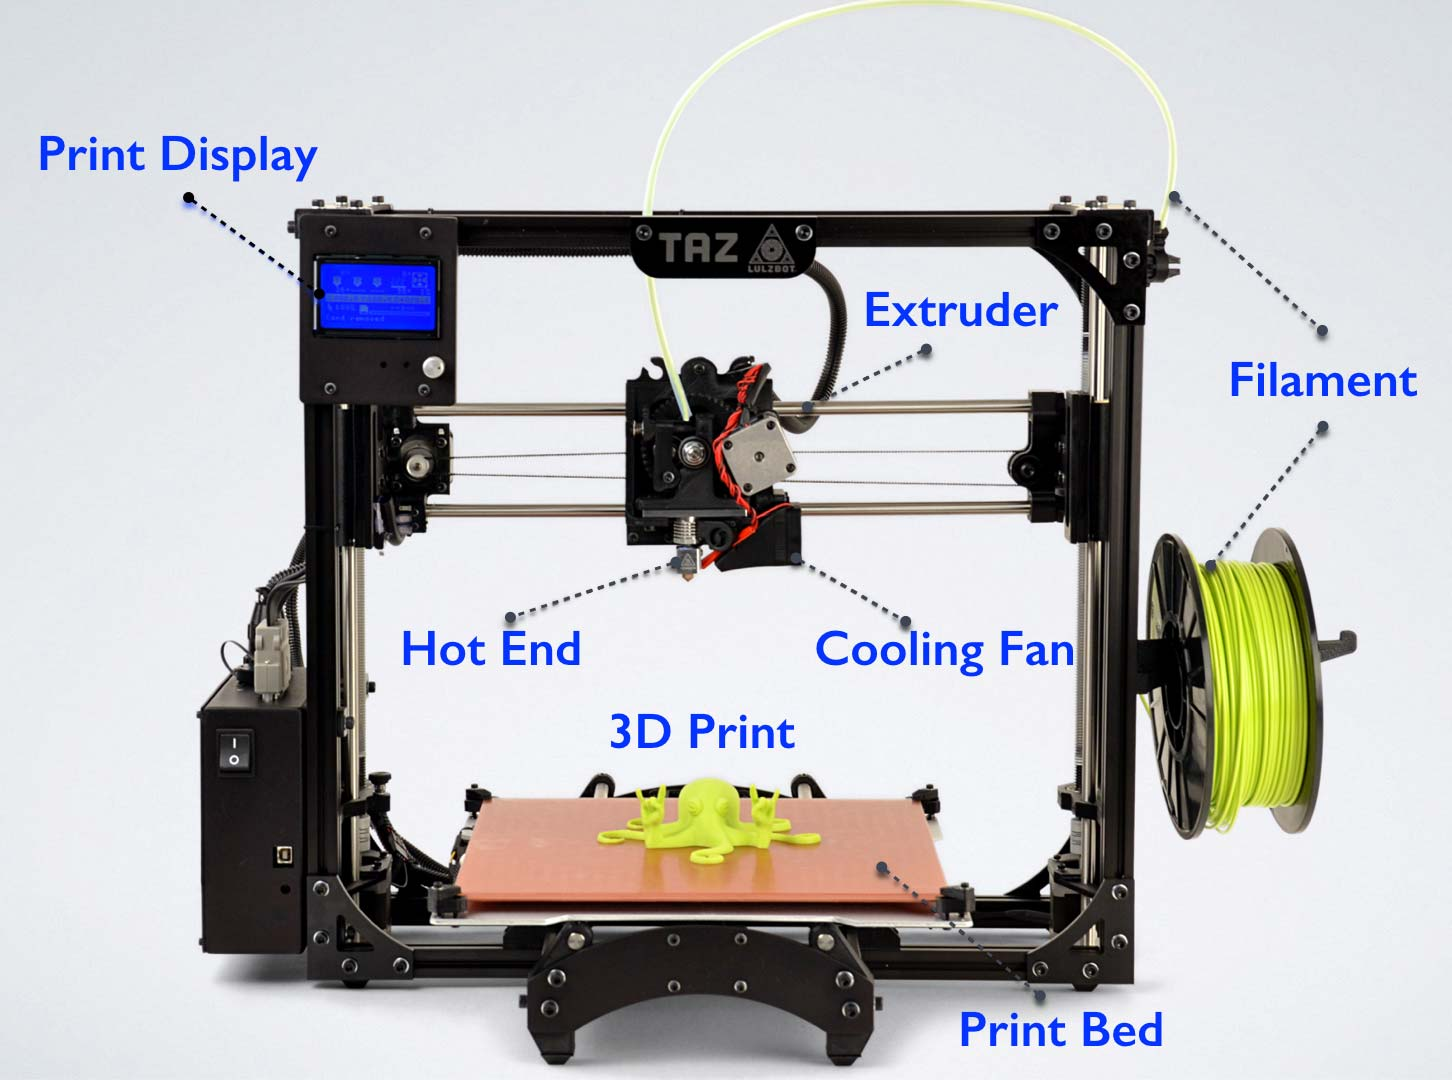
\includegraphics[scale=0.1]{Parts.jpg}
    \caption{Parts of a 3D printer}
    \label{fig:Parts}
\end{figure}

\section{Assumptions for modelling equations:}
The governing equations for the fluid flow and heat transfer were 
based on a continuum mixture model of \textit{Bennon and Incropera}. Additionally, the following assumptions were made: 

\begin{enumerate}
    \item The liquid and solid phases are modelled with a single fluid flow governing equation.

    \item The problem in the 2-D axis-symmetric coordinates and the buoyancy effect is incorporated by the Boussinesq's approximation. 

    \item Generalized Newtonian fluid was used above and below the glass transition temperature ($T_g$) (the temperature at which an amorphous polymer changes from a hard/glassy state to a soft/leathery state). So, the viscosity is made to be a function of temperature leading to very high values. Consequently, the melting filament behaves like a solid in the low-temperature region.

    \item \href{https://blog.rheosense.com/modeling-non-newtonian-fluids#:~:text=The%20Carreau%2DYasuda%20model%20is,Hackley%20and%20Ferraris%2C%202001)}{Carreau-Yasuda’s model} (emperical model, used to fit non-Newtonian data, describing pseudoplastic flow with asymptotic viscosities at zero and infinite shear rates, and with no yield stress) was used to model dynamic viscosity as follows: \[\eta = \frac{\eta_0 \alpha_T}{\left(1+(\lambda\alpha_T\gamma^.)^\alpha\right)^\frac{1-n}{\alpha}}\]
    where,
    \[a_T = exp\left(\frac{E_a}{R}\left(\frac{1}{T}-\frac{1}{T_{\infty}}\right)\right)\]
    
    $\eta_0$ is zero shear viscosity, $T_\infty$ is temp of ambient, $\gamma^.$ is effective shear rate, $\lambda$ is time constant, $\alpha_T$ is dimentionless temp dependence constant, a is dimentionless transition parameter, n is exponent.
    
    \item The densities of liquid and solid are not the same but are assumed to be constant in their respective phases.
    
    \item The liquidus temperature of the Acrylonitrile Butadiene Styrene (ABS) filament is 448 K (175 ℃). Though ABS is amorphous and doesn’t have a sharp melting temperature, but, it is usually printed at 20 K (20 ℃) higher than the melting temperature (428 K or 155 ℃) of Polyactic acid (PLA), another material for printing. In the current work, the solidus temperature of ABS is set to 433 K (160 ℃).

    \item The latent heat of fusion L is 0 J/kg. However, the current work assumes L to be a smaller value of 0.001 J/kg to predict the liquid-fraction evolution during melting.
\end{enumerate}

\section{Governing Equations:}
Non-dimensionalized governing equations for fluid flow are as follows:

\begin{enumerate}

    \item Continuity: \[\nabla (\vec{V}^*) = 0\]
    
    \item Momentum (derived from Navier-Stokes Equation): \[\frac{\partial\vec{V}^*}{\partial\tau} + \nabla(\vec{V}^*\cdot\vec{V}^*) = -\frac{1}{Re}\nabla P + \nabla\left(\frac{\eta^*}{Re} \frac{\rho}{\rho_l} \nabla(\vec{V}^*)\right) - \frac{\eta^*}{Re Da} \frac{\rho}{\rho_l}(\vec{V}^* - V^*_s) - \frac{Gr}{Re^2} T^* \]

    \item Energy (derived from Generalised Fourier's Equation): 
    \[\frac{\partial T^*}{\partial\tau} + \nabla(\vec{V}^* T^*) = \nabla \left({\frac{1}{Pe} \nabla T^*} \right) - \frac{f_s}{St} \nabla(\vec{V}^* - V^*_s) - \frac{f_l}{St}\nabla \vec{V}^* - \frac{1}{St} \frac{\partial{f_l}}{\partial \tau}+ Br\eta^* \left(\frac{\partial V_i}{\partial X_j} + \frac{\partial V_j}{\partial X_i}\right) \frac{\partial V_i}{\partial X_j}\]

\end{enumerate}

where ${V^*}$ is non-dimensionalized velocity and X is position coordinates, $\eta ^*$ is dynamic viscosity, $\tau$ is time, T is Temperature, Re is Reynolds number, P is pressure, $\rho$ is density, $\rho ^*_l$ is the density of the liquid, Da is Darcy number, Gr is Grashof number, Pe is Peclet number, Br is \href{https://en.wikipedia.org/wiki/Brinkman number#: ̃:text=It%20is%20the%20ratio%20between,the%20
larger%20the%20temperature%20rise}{Brinkman number} (the ratio of viscous heat generation to external heating) $\left(Br = \frac{\eta u^2}{\kappa(T_w-T_0)}\right)$, u is flow velocity, $\kappa$ is thermal conductivity, $T_0$ is bulk fluid temperature, $T_w$ is wall temperature St is Stephan number, $f_l$ is fraction of liquid.

\section{Interpreting Energy Equation}

The first term (conduction term) on the RHS of Energy eq. is reduced with an increase in Pe. The Pe's effect on the energy is similar to the effect of Re on the momentum equation. This increase in Pe reduces the conduction heat transfer term, making melting of the filament difficult.

The Stefan number (St) used in the present work is very large ($\approx$ 108), therefore, the St reduces the magnitude of the second to the fourth term on the RHS of eq. The large St is due to the low latent heat of the fusion L.

The contribution of these terms to heat transfer is negligibly small. In general, the St terms were not neglected in the current work since the liquid fraction $f_l$ helps to implement the heat boundary as shown in the later section. The last term on the RHS of Eq. becomes important only at higher Br.

\begin{figure}[!ht]
    \centering
    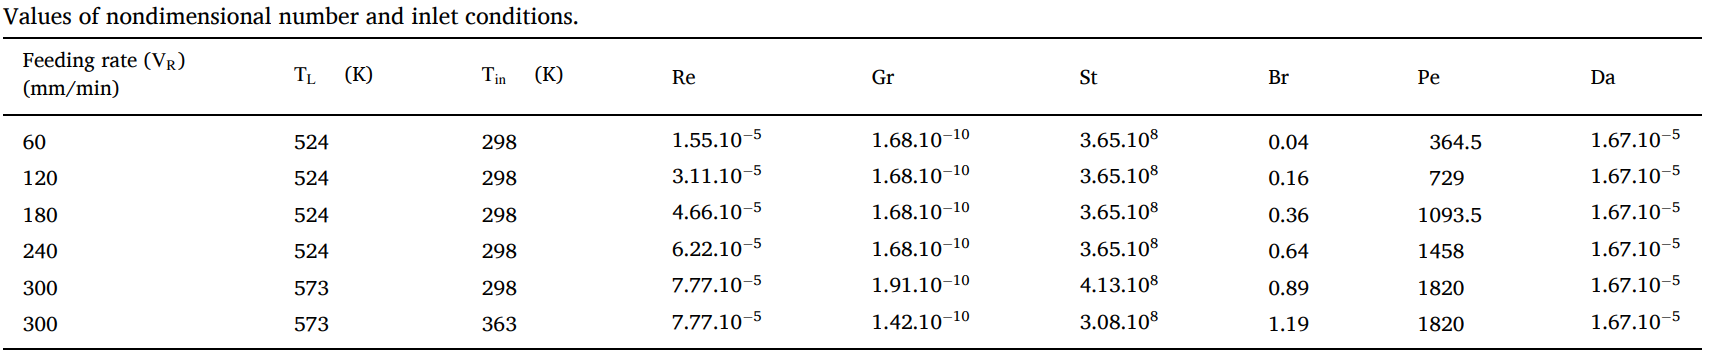
\includegraphics[scale=0.35]{Values.png}
    \caption{Values of non-dimensional numbers}
    \label{fig:Values}
\end{figure}

\section{System Analysis}

\begin{wrapfigure}{l}{0.25\textwidth}
    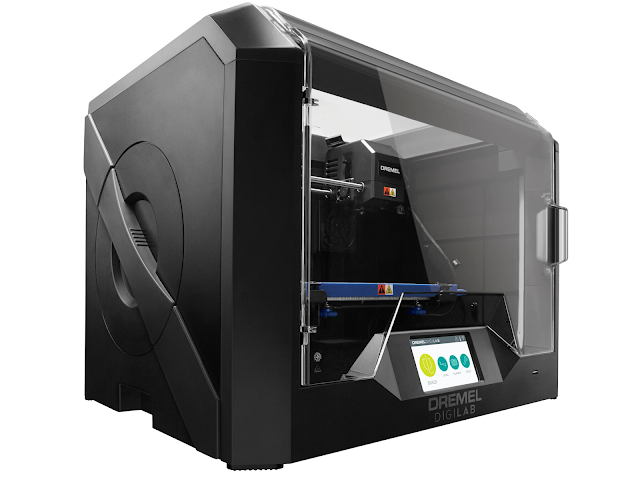
\includegraphics[width=1\linewidth]{printer.png}
    \caption{Dremel 3D45}
    \label{fig:Dremel 3D45}
\end{wrapfigure}

The system being studied is the hot end of the Dremel 3D45 printer. The diameter D of the heated barrel (with length $L_b$) is 2 mm, and the length $L_{capillary}$ = 0.5mm and diameter $d_{nozzle}$ = 0.4 mm of the capillary region of the nozzle. The solid ABS filament enters from the left (an inlet of the barrel) at a prescribed velocity and is extruded through the right (capillary region of the nozzle).

The boundary conditions used are:

\begin{enumerate}
    \item Zero gauge pressure at the nozzle exit (gauge pressure is the difference between the pressure in a system and the atmospheric pressure, as the nozzle and extruder are designed to operate at pressures close to atmosphere. When the 3D printer is operating, the pressure inside the system is almost equal to 1 atm, i.e. the gauge pressure is effectively zero).
    \item inlet velocity known as the feeding rate ${V_R}$ at the walls
    \item no-slip boundary conditions imposed
    \item at the exit of the liquefier the pressure outlet was used ($P_{out}$ = 0)
\end{enumerate}

\begin{wrapfigure}{r}{0.6\textwidth}
    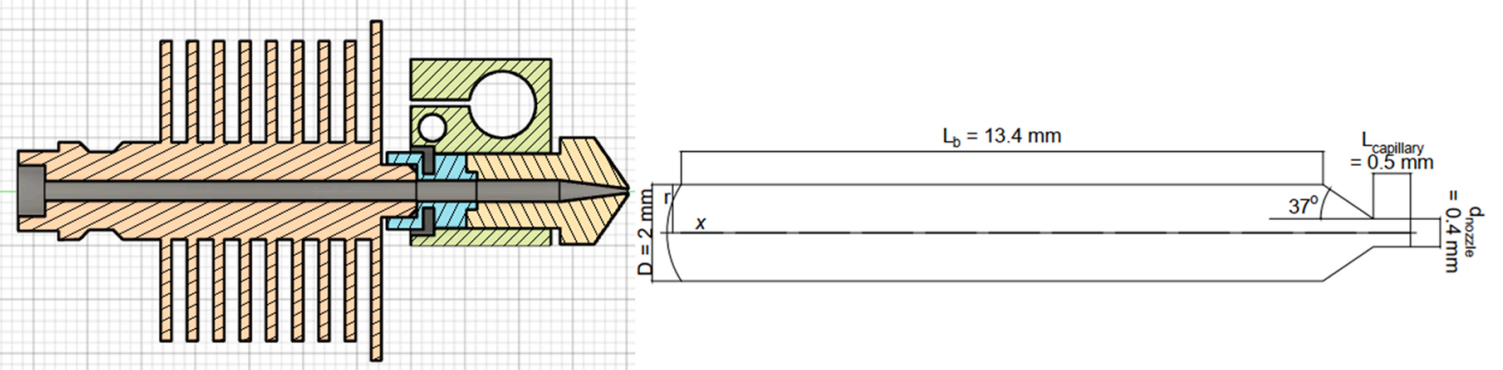
\includegraphics[width=1\linewidth]{Nozzel.png}
    \caption{Nozzel Diagram}
    \label{fig:Nozzel}
\end{wrapfigure}

Since there is no melt deposition onto a printing bed, the melt pressure at the exit of the capillary region of the nozzle can be neglected. The inlet temperature is set to $T_{in}$ as given in Table \ref{fig:Values} and the wall boundary condition is based on an energy balance between the inner surface of the channel and the filament: 

\[k\frac{\partial T}{\partial x} = h(T_L - T)\]
where h is the heat transfer coefficient and x is the direction vector towards nozzle.

\section{Solution to Equations:}

We declare our solution to be a steady state solution when the discrepancy of the velocity and temperature at the outlet of the domain being unsteady is less than 0.0003 $\%$ and 0.000025 $\%$ respectively. This convergence is achieved by continuous iterations.

We find the extrapolated axial velocity $u^{21}_{ext}$, approximate relative error $e^{21}_a$, the extrapolated relative error $e^{21}_{ext}$ and the Grid Convergence Index (GCI) using \href{https://www.sciencedirect.com/topics/mathematics/richardson-extrapolation#:~:text=The%20Richardson's%20extrapolation%20is%20a,of%20the%20solution%20is%20known}{Richardson extrapolation technique}. Table \ref{fig:GSA} shows that the error in governing equation by discretization is very small, the maximum being less than $2\%$ and it coincides with the centre of the nozzle and the minimum (0 value) is at the wall. So this is a valid method to proceed with.

\begin{figure}[!ht]
    \centering
    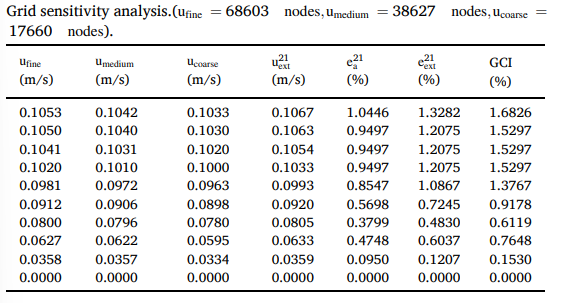
\includegraphics[scale=0.75]{Error table.png}
    \caption{Grid sensitivity analysis}
    \label{fig:GSA}
\end{figure}

\section{Effect of external parameters on the fluid and heat flow:}
\subsection{Effect of Specific heat capacity of filament}

\begin{wrapfigure}{r}{0.4\textwidth}
    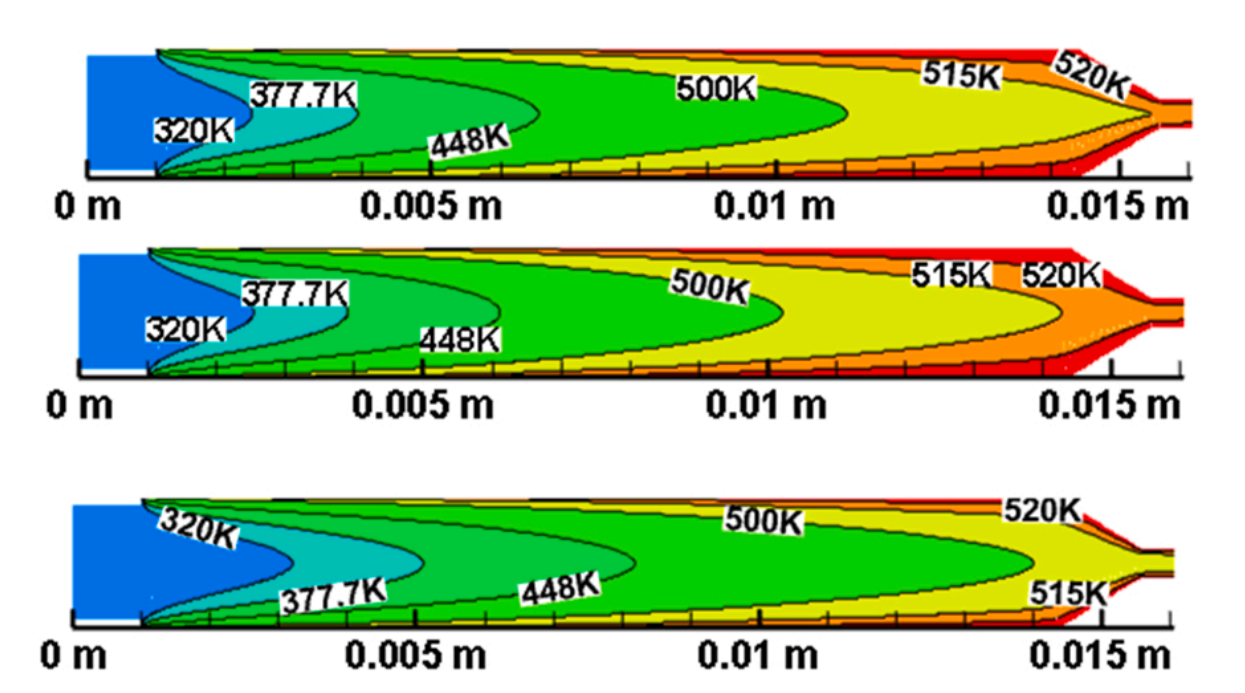
\includegraphics[width=1\linewidth]{T vs r contour.png}
    \caption{Contour plot for diff Cp's}
    \label{fig:Contour plot for diff Cp}
\end{wrapfigure}

The experimental results for specific heat capacity (Cp) of the filament, indicates that it is a temperature-proportional variable. The h was set to 104 W/(m2.K) at channel walls, $T_L$ = 523 K, $T_{in}$ =298 K and $V_R$ = 180 mm/min. 

\ref{fig:Contour plot for diff Cp} is a contour plot of the isotherms of the three values of Cp (The top plot is of $Cp_{F(T)}$ where F(T) is a function of temperature as $Cp_{F(T)} = 228.13 + 4.07T - 0.0026T^2$. This is a best-fit curve for experimental data for the given printer. The middle plot is of $Cp_{1470}$ and the bottom one is $Cp_{2100}$). 377.7 K isotherm is the glass transition temperature ($T_g$) (the temperature at which an amorphous polymer changes from a hard/glassy state to a soft/leathery state), and it is evident that the spatial position of the $T_g$ for the $Cp_{2100}$ is longer than the $Cp_{1470}$ and $Cp_{F(T)}$, as it brings more of the solid phase towards the nozzle exit.

\begin{figure}[!ht]
    \centering
    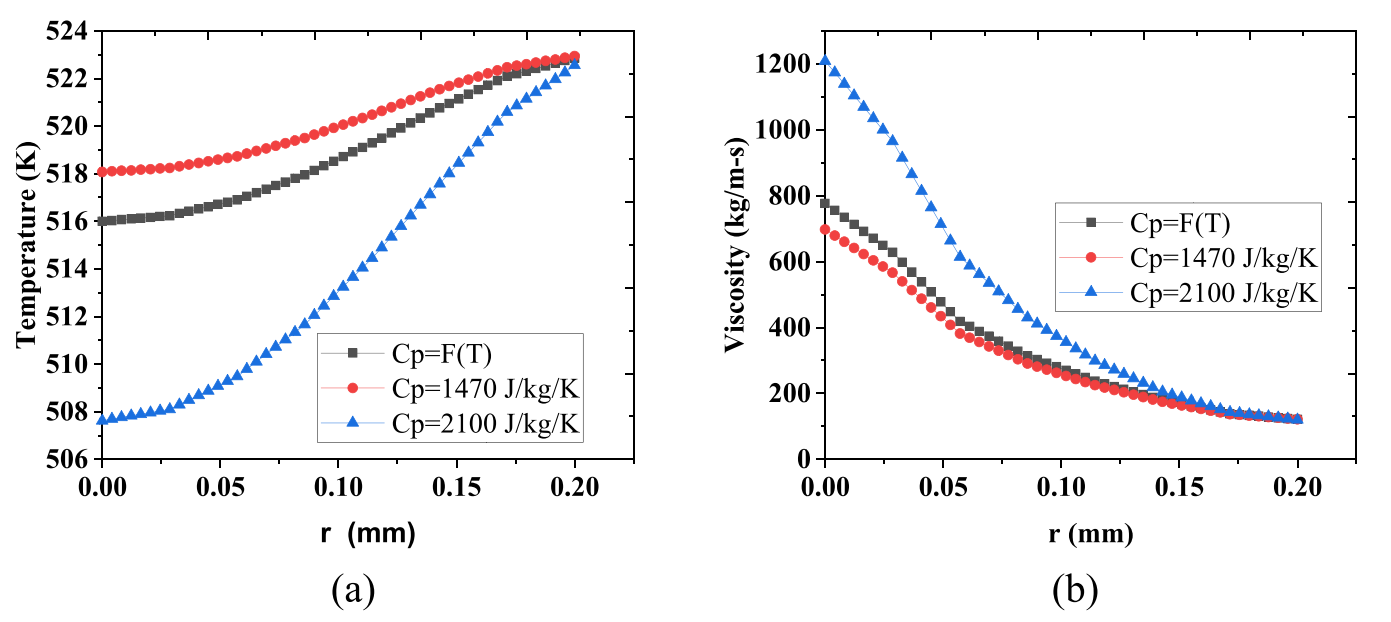
\includegraphics[scale=0.4]{T and mu vs r.png}
    \caption{Temp and viscosity vs r}
    \label{fig:T and mu vs r}
\end{figure}

Plot \ref{fig:T and mu vs r} shows that the temperature at the centre of the nozzle is below 508 K for the $Cp_{2100}$, 516 K and 518 K for the $Cp_{1470}$ and $Cp_{F(T)}$ respectively.

The viscosity is maximum at the nozzle centre with $Cp_{2100}$ having the highest value and falls monotonically towards the nozzle wall. In addition, the curve of the dynamic viscosity as shown for the $Cp_{F(T)}$ falls between the two curves giving a sense that the $Cp_{F(T)}$ is in the optimum range.

This flow is very similar to the \textbf{Hagen-Poiseulle flow} in the pipe where we had a parabolic shape of the velocity distribution with a maximum at the centre and minimum towards the wall due to the no-slip boundary condition.

The analytical equation used for \textbf{shear-thinning of a non-Newtonian 
fluid} can be found analytically using \[ u(r) = \frac{3n+1}{n+1} V_{avg} \left( 1-\left(\frac{r}{R}\right) ^{\left(\frac{1+n}{n}\right)} \right) \] where $V_{avg}$ is the average velocity of the fluid in the liquefier, r is the distance from the centre of the nozzle, R is the radius of the nozzle and n is the power index in the  \href{https://blog.rheosense.com/modeling-non-newtonian-fluids#:~:text=The%20Carreau%2DYasuda%20model%20is,Hackley%20and%20Ferraris%2C%202001)}{Carreau-Yasuda’s equation} as mentioned in Section 2.1, point 4 too.

\subsection{Effect of barrel length}

\begin{wrapfigure}{r}{0.5\textwidth}
    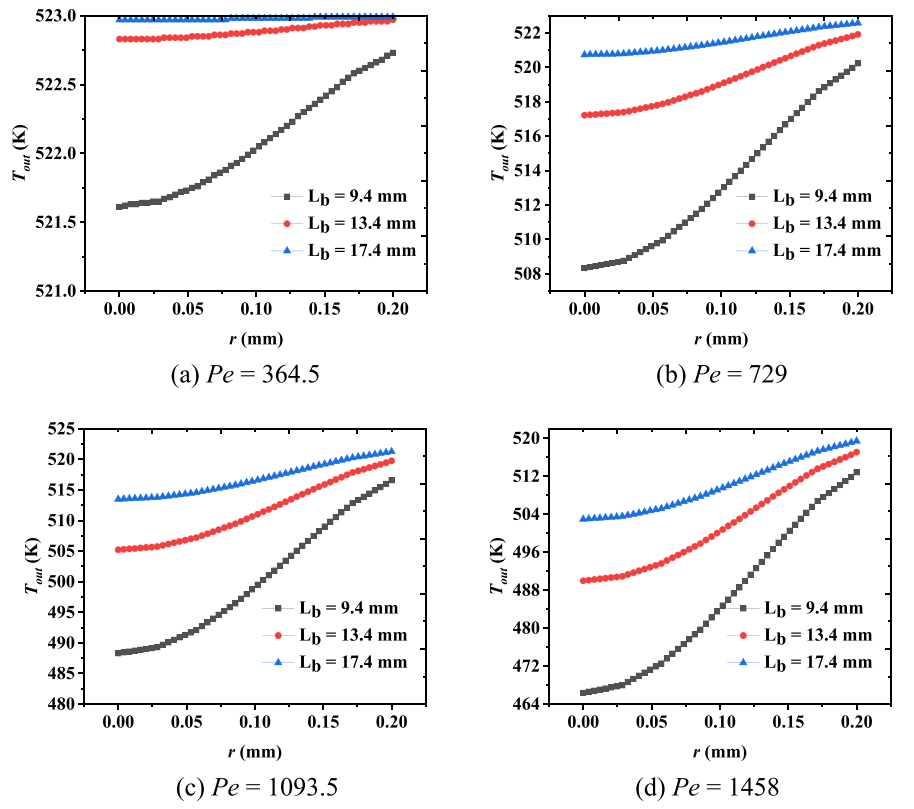
\includegraphics[width=1\linewidth]{Tout vs r.png}
    \caption{$T_{out}$ vs r}
    \label{fig:Tout vs r}
\end{wrapfigure}

The model discussed above had the presence of an air gap which gave rise to thermal resistance between the liquefier wall and the solid filament.

The net heat transfer coefficient is given as \[h_{net} = f_s h_{gap} + f_lh_c\]where $h_{gap}$ is the heat transfer coefficient at the air gap between the liquefier channel wall and the melting filament and $h_c$ is the heat transfer coefficient for the thermal wall contact between the molten filament and the wall. $f_s$ and $f_l$ are fractions of solid and liquid in the molten filament. It indicates that the solid region of the filament which has not melted, $h_{net}$ = $h_{gap}$ when $f_l = 0$ and as the melting proceeds $f_l$→1 then, h→$h_c$.

At the point of half melting, where $f_l = f_s = 0.5$, $h_{net}$ = $(h_{gap} + h_c)/2$. All of the above cases indicate that at the inlet of the channel, $h_{net}$ is minimum, due to no $f_l$. As the melting progresses, the molten filament is assumed to completely wet the walls of the liquefier channel, hence we get a higher value of $h_{net}$.

Plots \ref{fig:Tout vs r} presents the temperature at the output valve $T_{out}$ as a function of the radial distance from the nozzle from the centre for different Barrel lengths ($L_b$) and Peclet numbers (Pe) with $T_L$ = 523K.

Plots \ref{fig:Tout vs r}(a)-(b) shows that the longer the $L_b$ the lesser the drop in the $T_{out}$ at low Pe. This means that the $T_{out}$ is almost equal to the liquefier temperature for longer $L_b$ at low feeding rate.

However, the shorter $L_b$ shows a noticeable drop in the $T_{out}$ even at low Pe. The small drop in the previous case is due to the large heat transfer surface area and low Pe. This indicates that the heat transfer mechanism is mostly dominated by conduction for the longer $L_b$ than the shorter Lb.

Plots \ref{fig:Tout vs r}(b)-(d) also depicts the same trend as (a), but the temperature drop is more significant at the centre as the Pe increases. This decrease in temperature for shorter $L_b$ and increased feeding force increases the rate at which solid filament enters the heating chamber. Thus, it could not be sufficiently heated, enough to melt it.

\newpage

\begin{figure}[!ht]
    \centering
    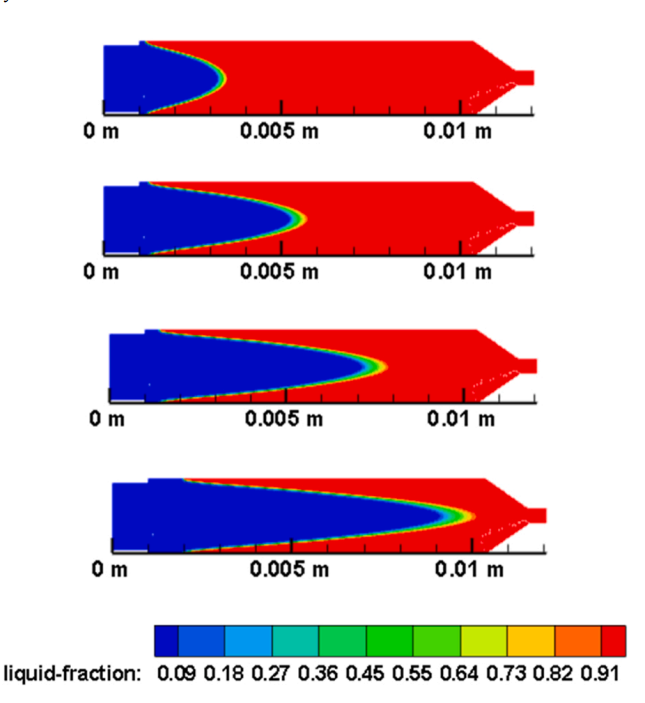
\includegraphics[scale=0.5]{Liq melting.png}
    \caption{Contour Plots}
    \label{fig:Liq Melting}
\end{figure}

Plot \ref{fig:Liq Melting} shows contour plots of the liquid fraction for various barrel lengths vs Pe. The blue-shaded region is a very low liquid fraction region, while the red region is the high liquid fraction region (fully melted filament). The liquid surface flows over the walls of the barrel easily at lower Pe, indicating that the starting of melting of the filament is the same for different barrel lengths and melting increases axially with the Peclet number.

\subsection{Effect of heating conditions}

When the initial temperature (65℃) of the filament was increased by 25℃ due to radiation from the heated barrel, i.e. it became 90℃, the temperature at outlet increased due to preheating of the solid filament. This may be associated with increased volumetric viscous heating with a higher Brinkman number (Br). It was observed that in the absence of preheating, the filament showed a mushy zone at the exit of nozzle of the liquefier suggesting that the melting of the solid filament was not completed before entering the nozzle.

\section{Conclusion}

It can be concluded that to optimize 3D printers, we can enable printing at high speeds and sufficiently high temperatures by increasing the heating section length. Experimental analysis indicates that printing at higher printing speed and with shorter barrel lengths could be viable if there are possibilities of preheating the feeding solid filament before entry into the barrel section. This enables us to build smaller 3D printers with the same capacity as larger ones, reducing cost and space. 

\chapter{Recent developments}
After analysing the various aspects of fluid and heat flow in a 3D printer, we shall now look at applications in practical domains of 3D Printers.

\section{Applications}
\begin{enumerate}
    \item \textbf{Circuit Boards}
    \\The conventional approach to producing an electric circuit board involves several steps, such as imaging, drilling, plating, solder mask coating, nomenclature printing, surface finishes, and using chemicals like acids and hard solvents. However, using 3D printing technology, polymer ink can be employed to create the board's layers, while silver polymer can produce the traces and holes necessary for electrical conduction. This method significantly reduces manufacturing time, particularly for intricate designs that would otherwise require weeks to complete through the traditional processes.
    
    \item \textbf{Health Industry}
    \\3D printing technology is being utilized to produce body parts for implants customized for an individual. They serve as replacements for completely failed components within the body. Various labs worldwide are using bio-compatible materials to develop bones, joints, ears, and noses, as well as internal organs like the heart, kidneys, blood vessels, etc. \\However, medical organizations have not yet authorized the use of such implants, as more time is required to evaluate their interactions with a living body.

    \item \textbf{Transportation industry}
    \\Complex engine and chassis parts in vehicles and turbine parts and airfoils for aircraft are successfully 3D printed for rapid prototyping. However, due to security reasons, these parts are not being used for mass production for the public yet, which would take a couple of years yet.

    \begin{figure}[!ht]
        \centering
        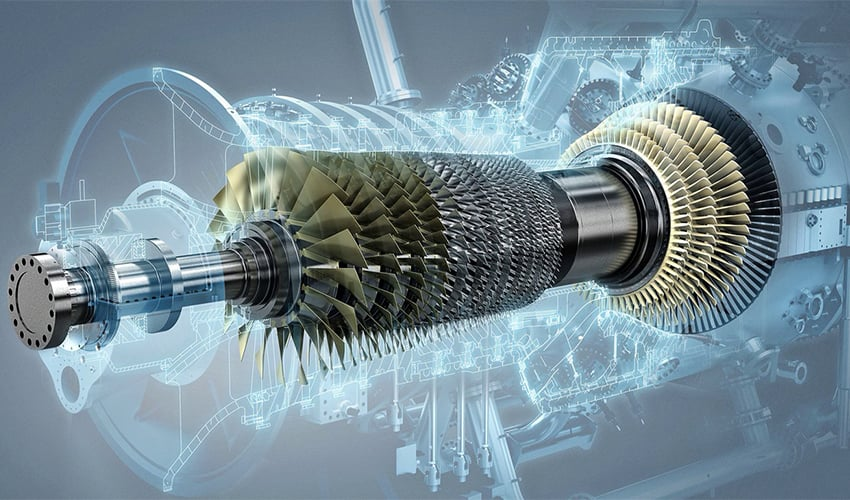
\includegraphics[scale=0.3]{Gas turbine.jpg}
        \caption{3D Printable design of a Gas turbine Engine}
        \label{fig:Gas Turbine Engine}
    \end{figure}

    \newpage
    \item \textbf{Education sector}
    \\The open-sourcing of 3D printing technology has made it accessible in local schools, numerous higher education institutions, and public libraries. The 'STEM' (Science, Technology, Engineering, and Mathematics) revolution has significantly benefited from this advancement by offering students an entirely new outlook on manufacturing processes.

    \item \textbf{Replicating artifacts and historical buildings}
    \\The cultural heritage field uses 3D printers to reprint old damaged artefacts. Many European and North American Museums have purchased 3D printers and actively recreate missing pieces of their relics and archaeological monuments.

    \item \textbf{Fashion Industry}
    \\Clothing and apparel giants like Nike uses 3D printing for generating prototypes and personalised shoe manufacturing for athletes. 3D printed eye-wear is also getting popular due to the ability of personalisation for each person with on-demand custom fit and styling. Complicated designs in gold jewellery are being 3D printed currently. This technology holds the potential to transform present markets to \textbf{'Print it yourself'} markets, greatly reducing heavy expenditure on industries.
    
    \item \textbf{Food Industry}
    \\Chocolates, Candies and flat foods like pizza, are indeed printable layerwise thereby enabling us to produce many exciting shapes and forms of food items which are totally new and niche for the markets. This idea may cause disruption among present food markets again due to customisation. The proposal of 3D printable food for astronauts in space is also being considered by NASA.
    
\end{enumerate}

\section{New Developments}
\begin{enumerate}
    \item \textbf{Multi-Material 3D Printing}
    \\The existing 3D printers allow only one material to be printed at a time, limiting their potential applications which require integrating different materials in the same object. Multi-material 3D printing solves this problem by allowing objects of complex arrangements of materials to be manufactured using a single printer. In this process, the material must be specified for each voxel (3D printing pixel element) inside the final object volume and the printer having multiple nozzles (each with the filament of a separate material), prints the objects by reading our supplied data. Though complicated to produce such machines, we would be able to revolutionise the entire domain of manufacturing with this new concept.
    
    \item \textbf{4D printing}
    4D printing is an additive manufacturing process in which the printed object transforms itself with the influence of stimuli like time, temperature, light, etc. It allows manufacturing of dynamic structures with adjustable shapes, properties or functionality. The smart stimulus-responsive materials created using 4D printing can be activated to create calculated responses such as self-assembly, self-repair, multi-functionality and shape-shifting. This allows for customized printing of shape-changing and shape-memory materials. It can thus help us to create alloys that were not viable before with extremely high precision.
\end{enumerate}

\begin{thebibliography}{9}
    \item Et. C.O. Ufodike and G.C. Nzebuka (2021), \url{https://doi.org/10.1016/j.addma.2021.102502}

    \item PIERRE J. CARREAU - TRANSACTIONS OF THE SOCIETY OF RHEOLOGY 16: 1, 99-127 (1972), \url{https://doi.org/10.1122/1.549276}
    

    \item \url{https://www.sciencedirect.com/topics/mathematics/richardson-extrapolation#:~:text=The%20Richardson's%20extrapolation%20is%20a,of%20the%20solution%20is%20known.}
    

    \item \url{https://blog.rheosense.com/modeling-non-newtonian-fluids#:~:text=The%20Carreau%2DYasuda%20model%20is,Hackley%20and%20Ferraris%2C%202001)}

    \item \url{https://www.lpfrg.com/guides/3d-printing-concepts-and-3d-printer-parts/}

    \item \url{https://solectroshop.com/en/blog/3d-printers-components-how-3d-printers-work-n40}
    
\end{thebibliography}

\end{document}